\documentclass[11pt,a4paper,sans,english]{moderncv}        % possible options include font size ('10pt', '11pt' and '12pt'), paper size ('a4paper', 'letterpaper', 'a5paper', 'legalpaper', 'executivepaper' and 'landscape') and font family ('sans' and 'roman')
\moderncvstyle{casual}                             % style options are 'casual' (default), 'classic', 'oldstyle' and 'banking'
\moderncvcolor{blue}                               % color options 'blue' (default), 'orange', 'green', 'red', 'purple', 'grey' and 'black'
%\nopagenumbers{}                                  % uncomment to suppress automatic page numbering for CVs longer than one page
\usepackage[utf8]{inputenc}                       % if you are not using xelatex ou lualatex, replace by the encoding you are using
\usepackage[scale=0.85,top=1cm, a4paper]{geometry}
\usepackage{babel}
\usepackage{tikz}
\usepackage{pgfgantt}
%----------------------------------------------------------------------------------
%            personal data
%----------------------------------------------------------------------------------
\renewcommand*{\namefont}{\fontsize{38}{40}\mdseries\upshape}
\firstname{Mitchell}
\familyname{Hansen}                             % optional, remove/comment the line if not wanted
\address{602 N. Pine St.}{Ellensburg, WA}{USA}         % optional, remove/comment the line if not wanted; the "country" arguments can be omitted or provided empty
\mobile{509-607-0079}                          % optional, remove/comment the line if not wanted
\email{mitchellhansen0@gmail.com}                               % optional, remove/comment the line if not wanted
\homepage{mitchellhansen.info}                         % optional, remove/comment the line if not wanted
\extrainfo{\homepagesymbol\httplink{github.com/mitchellhansen}}
% \photo[64pt][0.4pt]{picture}                       % optional, uncomment the line if wanted; '64pt' is the height the picture must be resized to, 0.4pt is the thickness of the frame around it (put it to 0pt for no frame) and 'picture' is the name of the picture file
%


\begin{document}
	
%-----       resume       ---------------------------------------------------------

\makecvtitle
\vspace*{-8mm}

\section{Education}
\cventry{2012--2017}{B.S. in Computer Science}{Central Washington University}{Ellensburg, WA}{}{}  % arguments 3 to 6 can be left empty
\section{Experience}
\subsection{Vocational}
\cventry{June 2016 -- Sept. 2016}{Full Stack Web Developer, Intern}{Donuts Inc.}{Bellevue}{}{At Donuts I created multiple sites utilizing the full web stack. From Javascript, HTML, and CSS, to Python, Flask, and AppEngine, I learned it all. Projects include a prototype link shortener, internal web page, a domain lookup landing page, and a realtime online game.}
\subsection{Miscellaneous}
\cventry{2009--2016}{Waiter}{The Palace Cafe}{Ellensburg, WA}{}{At the Palace I learned about teamwork, commitment, and responsibility.}


\section{Skills \& Languages}

\vspace*{-1mm}

\begin{minipage}{0.6\textwidth}
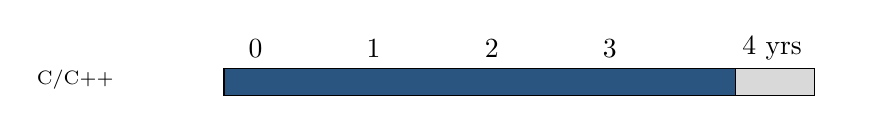
\begin{tikzpicture}
\draw[->,color=white, text=black] (2.9,0.6) -- (10.4,0.6) node[pos=0]{0} node[pos=0.2]{1} node[pos=0.4]{2} node[pos=0.6]{3} node[pos=0.875]{4 yrs};

\node [anchor=west] at (0,0.2) {\scriptsize{C/C++}};
\draw [fill=white!70!gray] (2.5,0) rectangle (10,.35);
\draw [fill={rgb:red,1;green,2;blue,3}] (2.5,0) rectangle (9,.35);
\end{tikzpicture}


\begin{tikzpicture}
\node [anchor=west] at (0,0.2) {\scriptsize{SFML}};
\draw [fill=white!70!gray] (2.5,0) rectangle (10,.35);
\draw [fill={rgb:red,1;green,2;blue,3}] (2.5,0) rectangle (7.5,.35);
\end{tikzpicture}


\begin{tikzpicture}
\node [anchor=west] at (0,0.2) {\scriptsize{CMake}};
\draw [fill=white!70!gray] (2.5,0) rectangle (10,.35);
\draw [fill={rgb:red,1;green,2;blue,3}] (2.5,0) rectangle (5.8,.35);
\end{tikzpicture}


\begin{tikzpicture}
\node [anchor=west] at (0,0.2) {\scriptsize{3D Graphics}};
\draw [fill=white!70!gray] (2.5,0) rectangle (10,.35);
\draw [fill={rgb:red,1;green,2;blue,3}] (2.5,0) rectangle (6,.35);
\end{tikzpicture}


\begin{tikzpicture}
\node [anchor=west] at (0,0.2) {\scriptsize{OpenCL}};
\draw [fill=white!70!gray] (2.5,0) rectangle (10,.35);
\draw [fill={rgb:red,1;green,2;blue,3}] (2.5,0) rectangle (5.5,.35);
\end{tikzpicture}


\begin{tikzpicture}
\node [anchor=west] at (0,0.2) {\scriptsize{C\# \& Java}};
\draw [fill=white!70!gray] (2.5,0) rectangle (10,.35);
\draw [fill={rgb:red,1;green,2;blue,3}] (2.5,0) rectangle (6,.35);
\end{tikzpicture}


\begin{tikzpicture}
\node [anchor=west] at (0,0.2) {\scriptsize{HTML \& CSS}};
\draw [fill=white!70!gray] (2.5,0) rectangle (10,.35);
\draw [fill={rgb:red,1;green,2;blue,3}] (2.5,0) rectangle (5,.35);
\end{tikzpicture}


\begin{tikzpicture}
\node [anchor=west] at (0,0.2) {\scriptsize{Javascript}};
\draw [fill=white!70!gray] (2.5,0) rectangle (10,.35);
\draw [fill={rgb:red,1;green,2;blue,3}] (2.5,0) rectangle (4.5,.35);
\end{tikzpicture}


\begin{tikzpicture}
\node [anchor=west] at (0,0.2) {\scriptsize{Python}};
\draw [fill=white!70!gray] (2.5,0) rectangle (10,.35);
\draw [fill={rgb:red,1;green,2;blue,3}] (2.5,0) rectangle (5.5,.35);
\end{tikzpicture}


\begin{tikzpicture}
\node [anchor=west] at (0,0.2) {\scriptsize{SQL}};
\draw [fill=white!70!gray] (2.5,0) rectangle (10,.35);
\draw [fill={rgb:red,1;green,2;blue,3}] (2.5,0) rectangle (4.5,.35);
\end{tikzpicture}


\begin{tikzpicture}
\node [anchor=west] at (0,0.2) {\scriptsize{Android}};
\draw [fill=white!70!gray] (2.5,0) rectangle (10,.35);
\draw [fill={rgb:red,1;green,2;blue,3}] (2.5,0) rectangle (4,.35);
\end{tikzpicture}
\end{minipage}
\begin{minipage}{0.3\textwidth}
\textbf{Other Skills,} *Nix, AWS, Alexa, Algorithms, AppEngine, Bash, Clang, Flask, GCC, GDB, GPGPU, Git, \LaTeX, OpenGL, Unity3D, Vim, Windows, Windows Phone, Zune
\end{minipage}

\vspace*{-2mm}

\section{Portfolio}
\cventry{}{Volumetric Rendering Engine}{OpenCL, C++, SFML, RayCasting, 3D Math}{}{}{An experimental "From Scratch" volumetric rendering engine utilizing a voxel dataset organized in a sparse voxel octree, Blinn-Phong lighting, dynamic shadowing, texturing, and reflections, along with a TCP streaming Android controller. Presented at the CWU College Of The Sciences fair.}
\cventry{}{Conways Game of Life}{OpenCL, C++, SFML}{}{}{Completely in-core GPU Conways Game of Life simulator and accompanying RLE decoder.}
\cventry{}{Mandelbrot Renderer}{OpenCL, C++, SFML}{}{}{Completely in-core GPU Mandelbrot renderer and explorer based on Wikipedia's Mandelbrot rendering algorithm.}
\cventry{}{Optimization Algorithms}{C++, Computer Science Mathematics}{}{}{Implementation of 15 optimization test suite functions, and 9 popular mathematical optimization algorithms.}
\cventry{}{Project Euler}{Python, Computer Science Mathematics}{}{}{Combinatorics, discrete math, and other logic problems solved using Python.}
\cventry{}{A* Pathfinding Implementation}{C++, SFML}{}{}{}
\end{document}
